\chapter{Introdu��o}

\section{Motiva�{\~ a}o}

\begin{figure}[ht]
\centering
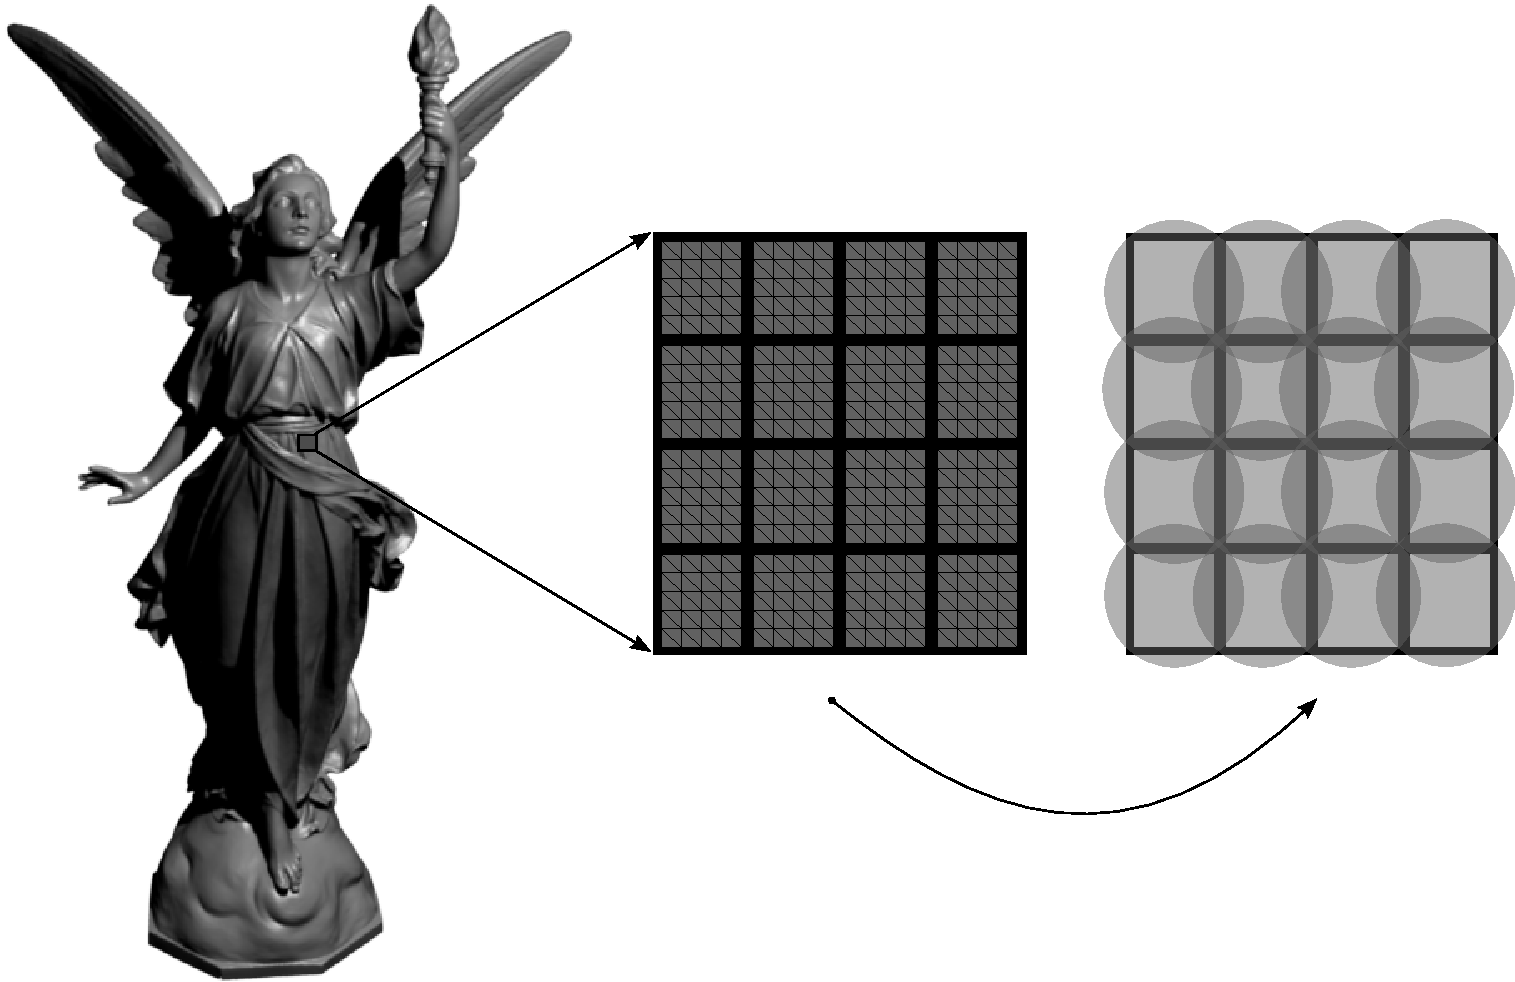
\includegraphics[width=16.0cm]{img/cap01/lucyIo} 
\caption{Lucy figure}
\label{fig:merge}
\end{figure}

\section{Renderiza��o Baseada em Pontos}
\section{N�vel de Detalhes}
\section{Objetivo}

\begin{algorithm}
\begin{algorithmic}[C]
\label{Algorithm:PQ}
\caption{Primeiro}
\IF {$i\geq maxval$} 
        \STATE $i\gets 0$
\ELSE
        \IF {$i+k\leq maxval$}
                \STATE $i\gets i+k$
        \ENDIF
\ENDIF 
\end{algorithmic}
\end{algorithm}

\section{Organiza�{\~ a}o da Disserta��o}

\begin{algorithm}
\begin{algorithmic}[C]
\label{Algorithm:PQ}
\caption{Segundo}
\IF {$i\geq maxval$} 
        \STATE $i\gets 0$
\ELSE
        \IF {$i+k\leq maxval$}
                \STATE $i\gets i+k$
        \ENDIF
\ENDIF 
\end{algorithmic}
\end{algorithm}
